%Version 3.1 December 2024
% See section 11 of the User Manual for version history
%
%%%%%%%%%%%%%%%%%%%%%%%%%%%%%%%%%%%%%%%%%%%%%%%%%%%%%%%%%%%%%%%%%%%%%%
%%                                                                 %%
%% Please do not use \input{...} to include other tex files.       %%
%% Submit your LaTeX manuscript as one .tex document.              %%
%%                                                                 %%
%% All additional figures and files should be attached             %%
%% separately and not embedded in the \TeX\ document itself.       %%
%%                                                                 %%
%%%%%%%%%%%%%%%%%%%%%%%%%%%%%%%%%%%%%%%%%%%%%%%%%%%%%%%%%%%%%%%%%%%%%

%%\documentclass[referee,sn-basic]{sn-jnl}% referee option is meant for double line spacing

%%=======================================================%%
%% to print line numbers in the margin use lineno option %%
%%=======================================================%%

%%\documentclass[lineno,pdflatex,sn-basic]{sn-jnl}% Basic Springer Nature Reference Style/Chemistry Reference Style

%%=========================================================================================%%
%% the documentclass is set to pdflatex as default. You can delete it if not appropriate.  %%
%%=========================================================================================%%

%%\documentclass[sn-basic]{sn-jnl}% Basic Springer Nature Reference Style/Chemistry Reference Style

%%Note: the following reference styles support Namedate and Numbered referencing. By default the style follows the most common style. To switch between the options you can add or remove "Numbered" in the optional parenthesis. 
%%The option is available for: sn-basic.bst, sn-chicago.bst%  
 
\documentclass[pdflatex,sn-nature]{sn-jnl}% Style for submissions to Nature Portfolio journals
%%\documentclass[pdflatex,sn-basic]{sn-jnl}% Basic Springer Nature Reference Style/Chemistry Reference Style
%%\documentclass[pdflatex,sn-mathphys-num]{sn-jnl}% Math and Physical Sciences Numbered Reference Style
%%\documentclass[pdflatex,sn-mathphys-ay]{sn-jnl}% Math and Physical Sciences Author Year Reference Style
%%\documentclass[pdflatex,sn-aps]{sn-jnl}% American Physical Society (APS) Reference Style
%%\documentclass[pdflatex,sn-vancouver-num]{sn-jnl}% Vancouver Numbered Reference Style
%%\documentclass[pdflatex,sn-vancouver-ay]{sn-jnl}% Vancouver Author Year Reference Style
%%\documentclass[pdflatex,sn-apa]{sn-jnl}% APA Reference Style
%%\documentclass[pdflatex,sn-chicago]{sn-jnl}% Chicago-based Humanities Reference Style

%%%% Standard Packages
%%<additional latex packages if required can be included here>

\usepackage{graphicx}%
\usepackage{multirow}%
\usepackage{amsmath,amssymb,amsfonts}%
\usepackage{amsthm}%
\usepackage{mathrsfs}%
\usepackage[title]{appendix}%
\usepackage{xcolor}%
\usepackage{textcomp}%
\usepackage{manyfoot}%
\usepackage{booktabs}%
\usepackage{algorithm}%
\usepackage{algorithmicx}%
\usepackage{algpseudocode}%
\usepackage{listings}%
\usepackage[nomarkers,figuresonly]{endfloat}% Move figures to the end
%%%%

%%%%%=============================================================================%%%%
%%%%  Remarks: This template is provided to aid authors with the preparation
%%%%  of original research articles intended for submission to journals published 
%%%%  by Springer Nature. The guidance has been prepared in partnership with 
%%%%  production teams to conform to Springer Nature technical requirements. 
%%%%  Editorial and presentation requirements differ among journal portfolios and 
%%%%  research disciplines. You may find sections in this template are irrelevant 
%%%%  to your work and are empowered to omit any such section if allowed by the 
%%%%  journal you intend to submit to. The submission guidelines and policies 
%%%%  of the journal take precedence. A detailed User Manual is available in the 
%%%%  template package for technical guidance.
%%%%%=============================================================================%%%%

%% as per the requirement new theorem styles can be included as shown below
\theoremstyle{thmstyleone}%
\newtheorem{theorem}{Theorem}%  meant for continuous numbers
%%\newtheorem{theorem}{Theorem}[section]% meant for sectionwise numbers
%% optional argument [theorem] produces theorem numbering sequence instead of independent numbers for Proposition
\newtheorem{proposition}[theorem]{Proposition}% 
%%\newtheorem{proposition}{Proposition}% to get separate numbers for theorem and proposition etc.

\theoremstyle{thmstyletwo}%
\newtheorem{example}{Example}%
\newtheorem{remark}{Remark}%

\theoremstyle{thmstylethree}%
\newtheorem{definition}{Definition}%

\raggedbottom
%%\unnumbered% uncomment this for unnumbered level heads

\begin{document}

\title[Bio-STFM]{Biology-constrained graph transformer bridges spatial transcriptomics and histopathology for interpretable cancer prognosis and in silico therapeutic hypothesis generation}

%%=============================================================%%
%% GivenName	-> \fnm{Joergen W.}
%% Particle	-> \spfx{van der} -> surname prefix
%% FamilyName	-> \sur{Ploeg}
%% Suffix	-> \sfx{IV}
%% \author*[1,2]{\fnm{Joergen W.} \spfx{van der} \sur{Ploeg} 
%%  \sfx{IV}}\email{iauthor@gmail.com}
%%=============================================================%%

\author[1,2,3]{\fnm{Dekang} \sur{Guo}}

\author[2,3]{\fnm{Yingying} \sur{Guo}}

\author[1]{\fnm{Xiaozhang} \sur{Liu}}

\author*[4]{\fnm{Jinke} \sur{Cheng}}\email{jkcheng@shsmu.edu.cn}

\author*[2,3]{\fnm{Qian} \sur{Han}}\email{qianhan@hainanu.edu.cn}

\affil[1]{\orgdiv{School of Computer Science and Technology}, \orgname{Hainan University}, \orgaddress{\city{Haikou}, \state{Hainan}, \postcode{570228}, \country{China}}}

\affil[2]{\orgdiv{Laboratory of Tropical Veterinary Medicine and Vector Biology, School of Life and Health Sciences, Hainan Province Key Laboratory of One Health, Collaborative Innovation Center of Life and Health}, \orgname{Hainan University}, \orgaddress{\city{Haikou}, \state{Hainan}, \postcode{570228}, \country{China}}}

\affil*[3]{\orgdiv{Hainan International One Health Institute}, \orgname{Hainan University}, \orgaddress{\city{Haikou}, \state{Hainan}, \country{China}}}

\affil[4]{\orgname{Hainan Medical University, Hainan Academy of Medical Sciences}, \orgaddress{\city{Haikou}, \state{Hainan}, \postcode{571199}, \country{China}}}

%%==================================%%
%% Sample for unstructured abstract %%
%%==================================%%

\abstract{Spatially resolved transcriptomics provides unprecedented insight into the tumor microenvironment but lacks the sample sizes needed for robust clinical prediction, whereas large pathology cohorts offer statistical power without molecular resolution. Here we present Bio-STFM, a hierarchical graph transformer that bridges these modalities using biology-constrained attention and cross-domain transfer learning. The framework constructs multi-scale tissue graphs and constrains attention with protein--protein interaction and pathway knowledge bases, while domain adaptation transfers spatial--molecular relationships from research atlases to routine histopathology. Applied to 16,502 patients across 10 cancer types, Bio-STFM achieves strong prognostic performance (C-index = 0.76) and yields biologically meaningful spatial patterns. An in silico perturbation module enables systematic sensitivity analyses of candidate cell--cell and ligand--receptor interactions, with top-ranked targets showing concordance with CRISPR dependency screens and established immunotherapy targets. Bio-STFM provides a unified framework for interpretable risk prediction and therapeutic hypothesis prioritization from standard pathology workflows.}

\keywords{Spatial transcriptomics, Computational pathology, Graph neural networks, Biological priors, Survival prediction, Therapeutic target discovery, Cancer prognosis}

%%\pacs[JEL Classification]{D8, H51}

%%\pacs[MSC Classification]{35A01, 65L10, 65L12, 65L20, 65L70}

\maketitle

\section{Introduction}\label{sec1}

The tumor microenvironment (TME) orchestrates cancer progression through complex spatial interactions among malignant cells, immune infiltrates, and stromal components\cite{bib1,bib69}. Understanding how these interactions collectively determine clinical outcomes---including therapeutic response and patient survival---represents a fundamental challenge in precision oncology\cite{bib63}. While emerging spatially resolved technologies now enable molecular profiling at single-cell resolution within intact tissue architecture\cite{bib2,bib67}, translating these rich biological insights into actionable clinical predictions remains elusive.

This translational gap stems from a fundamental data paradox confronting computational pathology (Fig.~1b). On one hand, spatially resolved transcriptomics platforms such as MERFISH\cite{bib44}, Visium\cite{bib38,bib43}, and Xenium\cite{bib45} provide unprecedented molecular resolution, revealing the cellular composition and gene expression patterns that define functional tissue niches\cite{bib3,bib39}. However, these technologies remain expensive, technically demanding, and limited to research settings, resulting in cohorts of hundreds rather than thousands of patients---insufficient for robust prognostic modeling. On the other hand, large-scale clinical databases such as The Cancer Genome Atlas (TCGA)\cite{bib10} archive tens of thousands of patients with detailed survival annotations and routine hematoxylin and eosin (H\&E) stained slides. Yet these valuable repositories typically lack spatially resolved molecular measurements needed to dissect mechanism, offering tissue morphology without matched spatial gene expression or cell identity information.

Current computational approaches have largely addressed these data modalities in isolation. Multiple instance learning (MIL) methods for whole-slide image (WSI) analysis have achieved notable success in survival prediction by aggregating patch-level morphological features\cite{bib4,bib5,bib18,bib52}, yet these approaches treat WSIs as unstructured bags of patches, discarding the spatial relationships that define tissue organization. Graph-based methods explicitly model spatial context\cite{bib6,bib40} but remain limited to morphological features without molecular grounding. Methods leveraging spatial transcriptomics have illuminated cellular neighborhoods and gene programs associated with disease states\cite{bib7,bib8,bib61,bib79}, though they typically lack the sample sizes needed for reliable clinical prediction. Moreover, existing frameworks predominantly model correlations\cite{bib21,bib42,bib77}, limiting interpretability and the ability to systematically test mechanistic hypotheses in silico.

The absence of a unified framework that integrates spatial molecular information with large-scale clinical outcomes creates a fundamental barrier to mechanistic clinical translation. Without identifying which specific cell--cell interactions and spatial motifs are most predictive and biologically plausible, it is difficult to prioritize therapeutic hypotheses or design follow-up validation studies. Moreover, the inability to transfer knowledge from richly profiled research cohorts to standard clinical workflows limits the practical impact of spatial biology discoveries.

Here we introduce Bio-STFM (Biology-constrained Spatial Transformer Foundation Model), a hierarchical graph transformer framework designed to bridge spatially resolved transcriptomics and routine histopathology using biological priors and domain adaptation. Our approach addresses three key limitations of existing methods. First, we construct multi-scale tissue graphs that explicitly represent the hierarchical organization of tissue---from gene regulatory networks within cells, to cellular neighborhoods, to tissue-level spatial motifs (Fig.~1c). This representation naturally captures nested biological scales through which local molecular events influence systemic outcomes\cite{bib13,bib51}. Second, we introduce a knowledge-guided attention mask that constrains learned attention patterns using prior biological knowledge from protein--protein interaction (PPI) networks and pathway databases\cite{bib14,bib34}. This inductive bias encourages information propagation to follow curated biology, improving interpretability and generalization. Third, we develop a domain adaptation strategy\cite{bib73} that leverages richly profiled spatial transcriptomics data to ``teach'' the model spatial--molecular relationships, which can then be applied to routine H\&E images lacking paired spatial molecular annotations.

A distinguishing feature of our framework is its capacity for in silico perturbation analysis (Fig.~1d). Beyond risk prediction, Bio-STFM enables systematic perturbations that computationally ``block'' specific cell--cell interactions or molecular signals and quantify the resulting change in predicted risk\cite{bib66}. This capability provides a practical mechanism for prioritizing therapeutic hypotheses for downstream experimental follow-up\cite{bib64}.

We systematically validated Bio-STFM across 10 cancer types comprising 16,502 patients from TCGA\cite{bib10,bib11}, with external validation on independent cohorts. Our model achieves strong prognostic performance (C-index = 0.76 $\pm$ 0.04 in cross-validation) compared to state-of-the-art methods while providing interpretable biological insights\cite{bib62}. We demonstrate that high-attention regions correspond to prognostically relevant tissue structures, including immune exclusion barriers associated with poor outcomes\cite{bib70}. Candidate targets prioritized through in silico perturbation show concordance with established immunotherapy targets\cite{bib20,bib54} and CRISPR dependency data, with 83\% validated across independent functional screens.

Our work provides a framework for integrating spatial molecular biology with clinical prediction, enabling mechanistic interpretation and therapeutic hypothesis generation from standard pathology workflows. By bridging the resolution-scale gap between research and clinical data modalities, Bio-STFM provides a foundation for translating spatial biology discoveries into precision oncology.

\section{Results}\label{sec2}

\subsection{Framework overview}\label{subsec1}

Bio-STFM addresses the fundamental challenge of linking spatially resolved molecular information to clinical outcomes while enabling mechanistic interpretation and in silico perturbation (Fig.~1a). The framework comprises three interconnected modules. First, whole slide images (WSIs) are tessellated into 256$\times$256 pixel patches and encoded via a pretrained Vision Transformer (ViT-H/14, indicating the ``Huge'' variant with 14$\times$14 patch size\cite{bib47}; initialized with CONCH weights\cite{bib22}) to obtain patch-level embeddings. Paired single-cell or bulk RNA-seq data is processed through Geneformer\cite{bib9} to generate genomic embeddings. These modalities are integrated via a knowledge-guided co-attention mechanism\cite{bib60}, where the attention matrix is constrained by a biological mask derived from prior protein--protein interaction (PPI) networks (Fig.~2a).

The tissue microenvironment is represented as a hierarchical graph spanning three scales (Fig.~1c): gene regulatory networks (L0), cellular neighborhoods (L1), and tissue-level motifs (L2)\cite{bib37,bib50}. Cross-layer edges enable multi-scale message passing, while the biological attention mask constrains information flow to curated interactions. For clinical application, we developed a domain adaptation strategy that transfers spatial--molecular relationships learned from richly profiled atlases (HTAN)\cite{bib11} to routine H\&E images lacking paired spatial molecular annotations, thereby bridging the data paradox illustrated in Fig.~1b.

A distinguishing capability of our framework is in silico perturbation (Fig.~1d). The perturbation module computationally ``blocks'' specific cell--cell interactions by setting corresponding edge weights to zero, enabling quantification of each interaction's sensitivity with respect to predicted risk as $\Delta\text{Risk} = f(G) - f(G')$, where $G$ and $G'$ represent original and perturbed graphs respectively (Fig.~2c).

\subsection{Multi-scale graph construction and knowledge-guided masked attention}\label{subsec2}

A hierarchical graph representation was developed to capture tissue organization across biological scales (Fig.~2b)\cite{bib36,bib41}. At the gene layer (L0), nodes represent genes connected by regulatory relationships derived from established gene regulatory networks. The cell layer (L1) models cellular neighborhoods where nodes are individual cells connected by physical proximity (within a defined spatial radius) or functional interactions inferred from ligand-receptor co-expression\cite{bib49}. The tissue layer (L2) encodes higher-order spatial motifs---recurring patterns of cell communities identified through unsupervised clustering of local neighborhood compositions\cite{bib32}.

The knowledge-guided masked attention mechanism (Fig.~2a) represents a key architectural innovation. Standard transformer attention computes weights as $A = \text{Softmax}(QK^T/\sqrt{d})$, allowing dense information flow between all node pairs. We introduce a knowledge mask $M$ derived from PPI databases (STRING) and pathway annotations (Reactome), where $M_{ij} = -\infty$ if no curated biological relationship exists between nodes $i$ and $j$. The masked attention $A = \text{Softmax}(QK^T/\sqrt{d} + M)$ effectively zeros out attention weights for biologically unsupported interactions, constraining the model to learn patterns consistent with established molecular biology.

\subsection{Bio-STFM improves survival prediction performance}\label{subsec3}

We evaluated Bio-STFM against state-of-the-art methods for survival prediction using 5-fold cross-validation across six cancer types from TCGA (BRCA, LUAD, COAD, KIRC, LIHC, BLCA; Fig.~3h). Bio-STFM achieved a mean concordance index (C-index) of 0.76 $\pm$ 0.04 (mean $\pm$ s.d.), significantly outperforming MCAT\cite{bib6} (0.72 $\pm$ 0.04; $P_{\text{adj}}$ = 0.012, paired $t$-test with Bonferroni correction for 4 comparisons), Porpoise\cite{bib23} (0.70 $\pm$ 0.03; $P_{\text{adj}}$ = 0.002), TransMIL\cite{bib18} (0.67 $\pm$ 0.04; $P_{\text{adj}}$ = 0.002), and ABMIL\cite{bib4} (0.63 $\pm$ 0.03; $P_{\text{adj}}$ $<$ 0.001). This represents our primary benchmark with rigorous cross-validation ensuring unbiased performance estimates.

We further assessed performance on held-out test sets (20\% of each cohort) across an expanded panel of 10 cancer types (Fig.~3a). Bio-STFM achieved a sample-size weighted average C-index of 0.786, outperforming MCAT\cite{bib6} (0.665), Porpoise\cite{bib23} (0.662), TransMIL\cite{bib18} (0.621), CLAM-SB\cite{bib5} (0.620), ABMIL\cite{bib4} (0.596), and Mean-Pool baseline (0.563). The performance advantage was consistent across cancer types, with the largest improvements observed in breast cancer (BRCA) and lung adenocarcinoma (LUAD).

Kaplan-Meier analysis on the TCGA-BRCA cohort (n = 912 patients, 339 events) demonstrated that Bio-STFM-predicted risk groups showed significant survival separation (Fig.~3b). The high-risk group exhibited substantially worse outcomes compared to the low-risk group (hazard ratio [HR] = 3.14; 95\% confidence interval [CI]: 2.54--3.76; log-rank $P < 0.0001$). Median survival in the high-risk group was 28.3 months compared to 67.2 months in the low-risk group.

\subsection{External validation confirms generalizability}\label{subsec4}

To assess generalizability beyond the TCGA training cohort, we validated Bio-STFM on two independent publicly available datasets (Fig.~3c). The first external cohort comprised breast cancer samples from the Clinical Proteomic Tumor Analysis Consortium (CPTAC-BRCA; n = 122), which were collected and processed independently from TCGA with different tissue handling protocols and scanning equipment\cite{bibCPTAC}. The second external cohort was derived from held-out TCGA tissue source sites (TCGA-TSS; n = 285) representing geographically distinct institutions not included in training. Despite differences in patient demographics and technical variation, the model maintained robust risk stratification in both cohorts. CPTAC-BRCA showed significant survival separation (HR = 2.87; 95\% CI: 2.21--3.73; $P < 0.0001$) and TCGA-TSS demonstrated comparable performance (HR = 2.64; 95\% CI: 1.98--3.52; $P < 0.0001$), supporting generalizability across independent data sources.

Subgroup analysis across clinical covariates demonstrated consistent prognostic value (Fig.~3g). We stratified patients by age ($<$50, 50--65, $>$65 years), sex, tumor stage (I--II, III, IV), molecular subtype (Luminal A, Luminal B, HER2+, Triple-negative), and chemotherapy status. All subgroups showed HR $>$ 1, indicating that model-predicted risk remained prognostically informative regardless of clinical characteristics. The overall hazard ratio across 16,502 patients was 2.19 (95\% CI: 1.82--2.64), with the strongest effect observed in advanced-stage (III--IV) patients (HR = 2.78; 95\% CI: 2.15--3.59) and triple-negative breast cancer (HR = 2.91; 95\% CI: 2.18--3.88). The proportional hazards assumption was verified using Schoenfeld residual tests ($P$ = 0.34 for global test), confirming validity of the Cox model.

\subsection{Spatial expression prediction validates cross-modal learning}\label{subsec5}

A key hypothesis underlying our approach is that the model learns meaningful spatial-molecular relationships during pretraining on paired spatial transcriptomics data. To validate this, we assessed the model's ability to predict spatial gene expression from histopathology images (Fig.~3d). Comparing model predictions against ground-truth values from held-out Visium spatial transcriptomics data (n = 40,000 spots across 12 held-out samples), we observed substantial concordance with a median $R^2$ of 0.58 across 250 highly variable genes (interquartile range [IQR]: 0.42--0.71; Pearson $r$ = 0.76). This performance is comparable to or exceeds existing spatial prediction methods\cite{bib74,bib75} and demonstrates that the domain adaptation module effectively transfers spatial-molecular knowledge learned from HTAN data to routine H\&E images.

Expression predictions showed expected gene-specific variation related to morphological visibility. Genes with strong tissue-level expression patterns achieved the highest accuracy, including epithelial markers (KRT8, KRT18; $R^2$ = 0.72--0.78), immune markers (CD3E, CD8A; $R^2$ = 0.62--0.68), and stromal markers (VIM, COL1A1; $R^2$ = 0.58--0.65). Genes with diffuse expression patterns or low morphological correlates showed lower prediction accuracy ($R^2$ = 0.35--0.50), consistent with the biological expectation that H\&E morphology primarily captures cell-type composition rather than intracellular transcriptional states.

\subsection{Ablation studies quantify component contributions}\label{subsec6}

We performed systematic ablation experiments to quantify the contribution of each architectural component (Fig.~3e). Removing the domain bridge module resulted in the largest performance decrease ($\Delta$C-index = $-$0.057), confirming the importance of cross-modal knowledge transfer. The spatial graph structure contributed substantially ($\Delta$C-index = $-$0.052), demonstrating that explicit modeling of tissue topology provides information beyond unstructured patch aggregation. The knowledge mask showed meaningful impact ($\Delta$C-index = $-$0.042), indicating that biological prior knowledge improves model generalization. Masked tissue modeling (MTM) pretraining ($\Delta$C-index = $-$0.040) and hierarchical graph structure ($\Delta$C-index = $-$0.035) each provided additional gains. A random baseline lacking all components showed the largest drop ($\Delta$C-index = $-$0.136), underscoring the collective contribution of our architectural innovations.

These results support our hypothesis that integrating spatial structure, biological priors, and cross-modal learning provides complementary sources of information for survival prediction.

\subsection{Computational efficiency enables clinical deployment}\label{subsec7}

Practical clinical application requires efficient inference. We characterized computational requirements as a function of graph size on an NVIDIA RTX 4090 GPU (24GB; Fig.~3f). For typical WSIs generating graphs of 2,000--4,000 nodes, the model requires 8--15GB GPU memory and achieves throughput of 25--40 WSI per minute. At the recommended maximum graph size (5,000 nodes), memory consumption reaches 18GB with throughput of 20 WSI per minute. These characteristics enable deployment on standard clinical computing infrastructure, processing a typical daily pathology workload (200--500 slides) within minutes.

\subsection{Attention maps reveal biologically meaningful tissue patterns}\label{subsec8}

Beyond predictive performance, a central goal of Bio-STFM is interpretable identification of prognostically relevant tissue features. We visualized attention weights learned by the model on representative whole slide images (Fig.~4a). In a breast cancer case with predicted risk score 0.725 (high-risk), the model allocated highest attention to regions at the tumor-stroma interface and areas with specific immune cell configurations. Importantly, high attention indicates relevance for prediction rather than high risk per se; the model identifies tissue features informative for distinguishing patient outcomes.

To assess interpretation robustness, we performed perturbation stability analysis (Fig.~4b). We systematically perturbed model inputs using five strategies (noise injection, dropout, shuffle, edge removal, node removal) at varying intensities (1--50\%) and measured rank correlation between original and perturbed attention rankings. High correlations ($>$0.89) were maintained across most conditions, indicating that the model's interpretations are robust to input perturbations and not artifacts of overfitting. Significant degradation occurred only at extreme perturbation levels ($>$30\%), where input structure was substantially corrupted.

\subsection{Biological constraints improve attention interpretability}\label{subsec9}

We hypothesized that incorporating biological prior knowledge via the knowledge mask would produce more focused and interpretable attention patterns. To test this, we compared attention entropy---a measure of attention dispersion---across model variants (Fig.~4d). Lower entropy indicates concentrated attention on fewer regions, facilitating interpretation.

The full model achieved significantly lower attention entropy compared to ablated versions removing biological constraints ($P < 0.001$, two-sided Wilcoxon test), spatial structure ($P < 0.001$), or using random attention ($P < 0.001$). This pattern persisted across transformer layers (Fig.~4e): the full model maintained consistently lower entropy through layers 1, 3, and 6, while ablated variants showed progressively increasing entropy, particularly in deeper layers. These results demonstrate that biological and spatial constraints jointly promote focused, interpretable attention throughout the network hierarchy.

\subsection{Spatial motifs associate with patient survival}\label{subsec10}

Examination of high-attention regions revealed recurring cellular arrangements that we term spatial motifs. Figure~4c illustrates the cell community structure in a representative high-risk region, showing 400 cells colored by type (Tumor, CAF, CD8+ T cells, CD4+ T cells, Macrophages, B cells, Endothelial cells, NK cells). A notable pattern emerged: cancer-associated fibroblasts (CAFs) frequently formed barriers around CD8+ T cells, potentially preventing immune infiltration into tumor cores.

We formalized this observation as the ``immune exclusion barrier motif'' (Fig.~4f), characterized by CAF cells physically surrounding T cell populations\cite{bib56}. TGF$\beta$-TGFBR signaling was identified as the predominant mediator of this barrier\cite{bib56}. Patients harboring this motif showed significantly worse survival (HR = 2.15; $P$ = 0.001). Comparison of motif frequency between survival groups (Fig.~4g) confirmed that patients with short survival (n = 81) harbored significantly more immune exclusion motifs than those with long survival (n = 119; $P < 0.0001$, two-sided Mann-Whitney $U$ test).

\subsection{Gene expression correlates with morphological phenotypes}\label{subsec11}

The hierarchical graph structure enables analysis of relationships between molecular features and histopathological phenotypes. We computed correlations between marker gene expression levels and quantitative morphological features extracted from H\&E images (Fig.~4h).

Notable associations included: nuclear pleomorphism correlated with ERBB2 expression ($r = 0.62$; $P < 0.05$, Bonferroni-corrected) and TP53 expression ($r = 0.73$; $P < 0.05$); nuclear area correlated with TP53 ($r = 0.24$; $P < 0.05$); and stromal ratio correlated with VIM expression ($r = 0.31$; $P < 0.05$). These associations link specific molecular alterations to morphological phenotypes observable in routine H\&E staining, providing mechanistic insight into how genetic changes manifest as visible tissue changes.

\subsection{Virtual intervention identifies therapeutic targets}\label{subsec12}

A key capability of Bio-STFM is in silico perturbation analysis: computationally simulating the effect of blocking specific molecular interactions on predicted risk. We systematically screened cell-cell and ligand-receptor interactions by computing $\Delta$Risk for each interaction across the patient cohort (Fig.~5a).

Ranking interactions by predicted survival benefit revealed established therapeutic targets among top candidates, including CSF1R, CTLA4\cite{bib54,bib55}, PD1-PDL1\cite{bib20}, and TGF$\beta$1 pathways\cite{bib56}. Of the top 10 ranked interactions, 6 (60\%) corresponded to established therapeutic targets with approved drugs or advanced clinical trials, demonstrating the model's ability to rediscover known biology while prioritizing actionable candidates. The remaining 4 interactions represent novel therapeutic hypotheses warranting experimental validation.

To assess statistical significance, we performed permutation testing by randomly shuffling interaction labels and recomputing $\Delta$Risk values (Fig.~5e). Of the top 50 ranked targets, 45 (90\%) achieved statistical significance ($P < 0.05$) against the null distribution, confirming that the model's predictions represent genuine biological signals rather than chance findings.

\subsection{Perturbation-based survival sensitivity analysis}\label{subsec13}

Beyond target identification, Bio-STFM enables perturbation-based survival sensitivity analysis. Figure~5b illustrates this analysis for simulated PD1-PDL1 blockade. We selected high-risk patients (n = 200) and compared predicted survival curves under original conditions versus after computationally blocking the PD1-PDL1 interaction.

The perturbation analysis predicted a median survival separation of +4.8 months ($\Delta$Median; 95\% CI: 2.1--7.6 months; log-rank $P$ = 0.03) between baseline and perturbed predictions. Importantly, the predicted effect was heterogeneous: patients with high baseline PD-L1 expression showed larger predicted separation (+6.2 months) compared to PD-L1-low patients (+2.1 months), recapitulating known biomarker associations.

We further analyzed predicted tumor microenvironment (TME) state transitions upon virtual treatment (Fig.~5c). Using UMAP visualization, patients were distributed across four TME phenotypes: Cold (immune-desert), Intermediate, Hot (immune-infiltrated), and Responder. Virtual PD1-PDL1 blockade predicted transitions from Cold/Intermediate toward Hot/Responder phenotypes, with an overall response rate of 57/150 patients (38\%). This predicted response rate closely matches observed immunotherapy response rates in breast cancer clinical trials (35--42\%), providing additional validation of the model's biological plausibility.

\subsection{External validation confirms target biological relevance}\label{subsec14}

To validate the biological relevance of model-identified targets, we cross-referenced our predictions against three independent evidence sources (Fig.~5d): CRISPR dependency screens (DepMap), drug sensitivity assays, and clinical trial outcomes. For the top 8 ranked targets (PD1, EGFR, HER2, CTLA4, VEGFA, CSF1R, TGF$\beta$1, LAG3), we observed 7 of 8 (87.5\%) validated by CRISPR screens, 6 of 8 (75\%) by drug sensitivity data, and 8 of 8 (100\%) concordance with clinical evidence. Notably, 6 of 8 targets have FDA-approved therapies, with the remaining 2 (CSF1R, LAG3) in Phase III clinical trials.

Quantitative analysis of target overlap with external databases (Fig.~5f) showed that of 23 model-identified targets, 19 (83\%) were validated by CRISPR DepMap screens, 18 (78\%) by DrugBank annotations, and 15 (65\%) by clinical trial registrations. Twelve targets (52\%) were validated by all three sources, demonstrating strong concordance across orthogonal evidence types. This convergent validation supports both the biological validity and translational potential of Bio-STFM for therapeutic hypothesis generation.

%%==============================%%
%%  Main Figures                %%
%%==============================%%

\begin{figure}[!htbp]
\centering
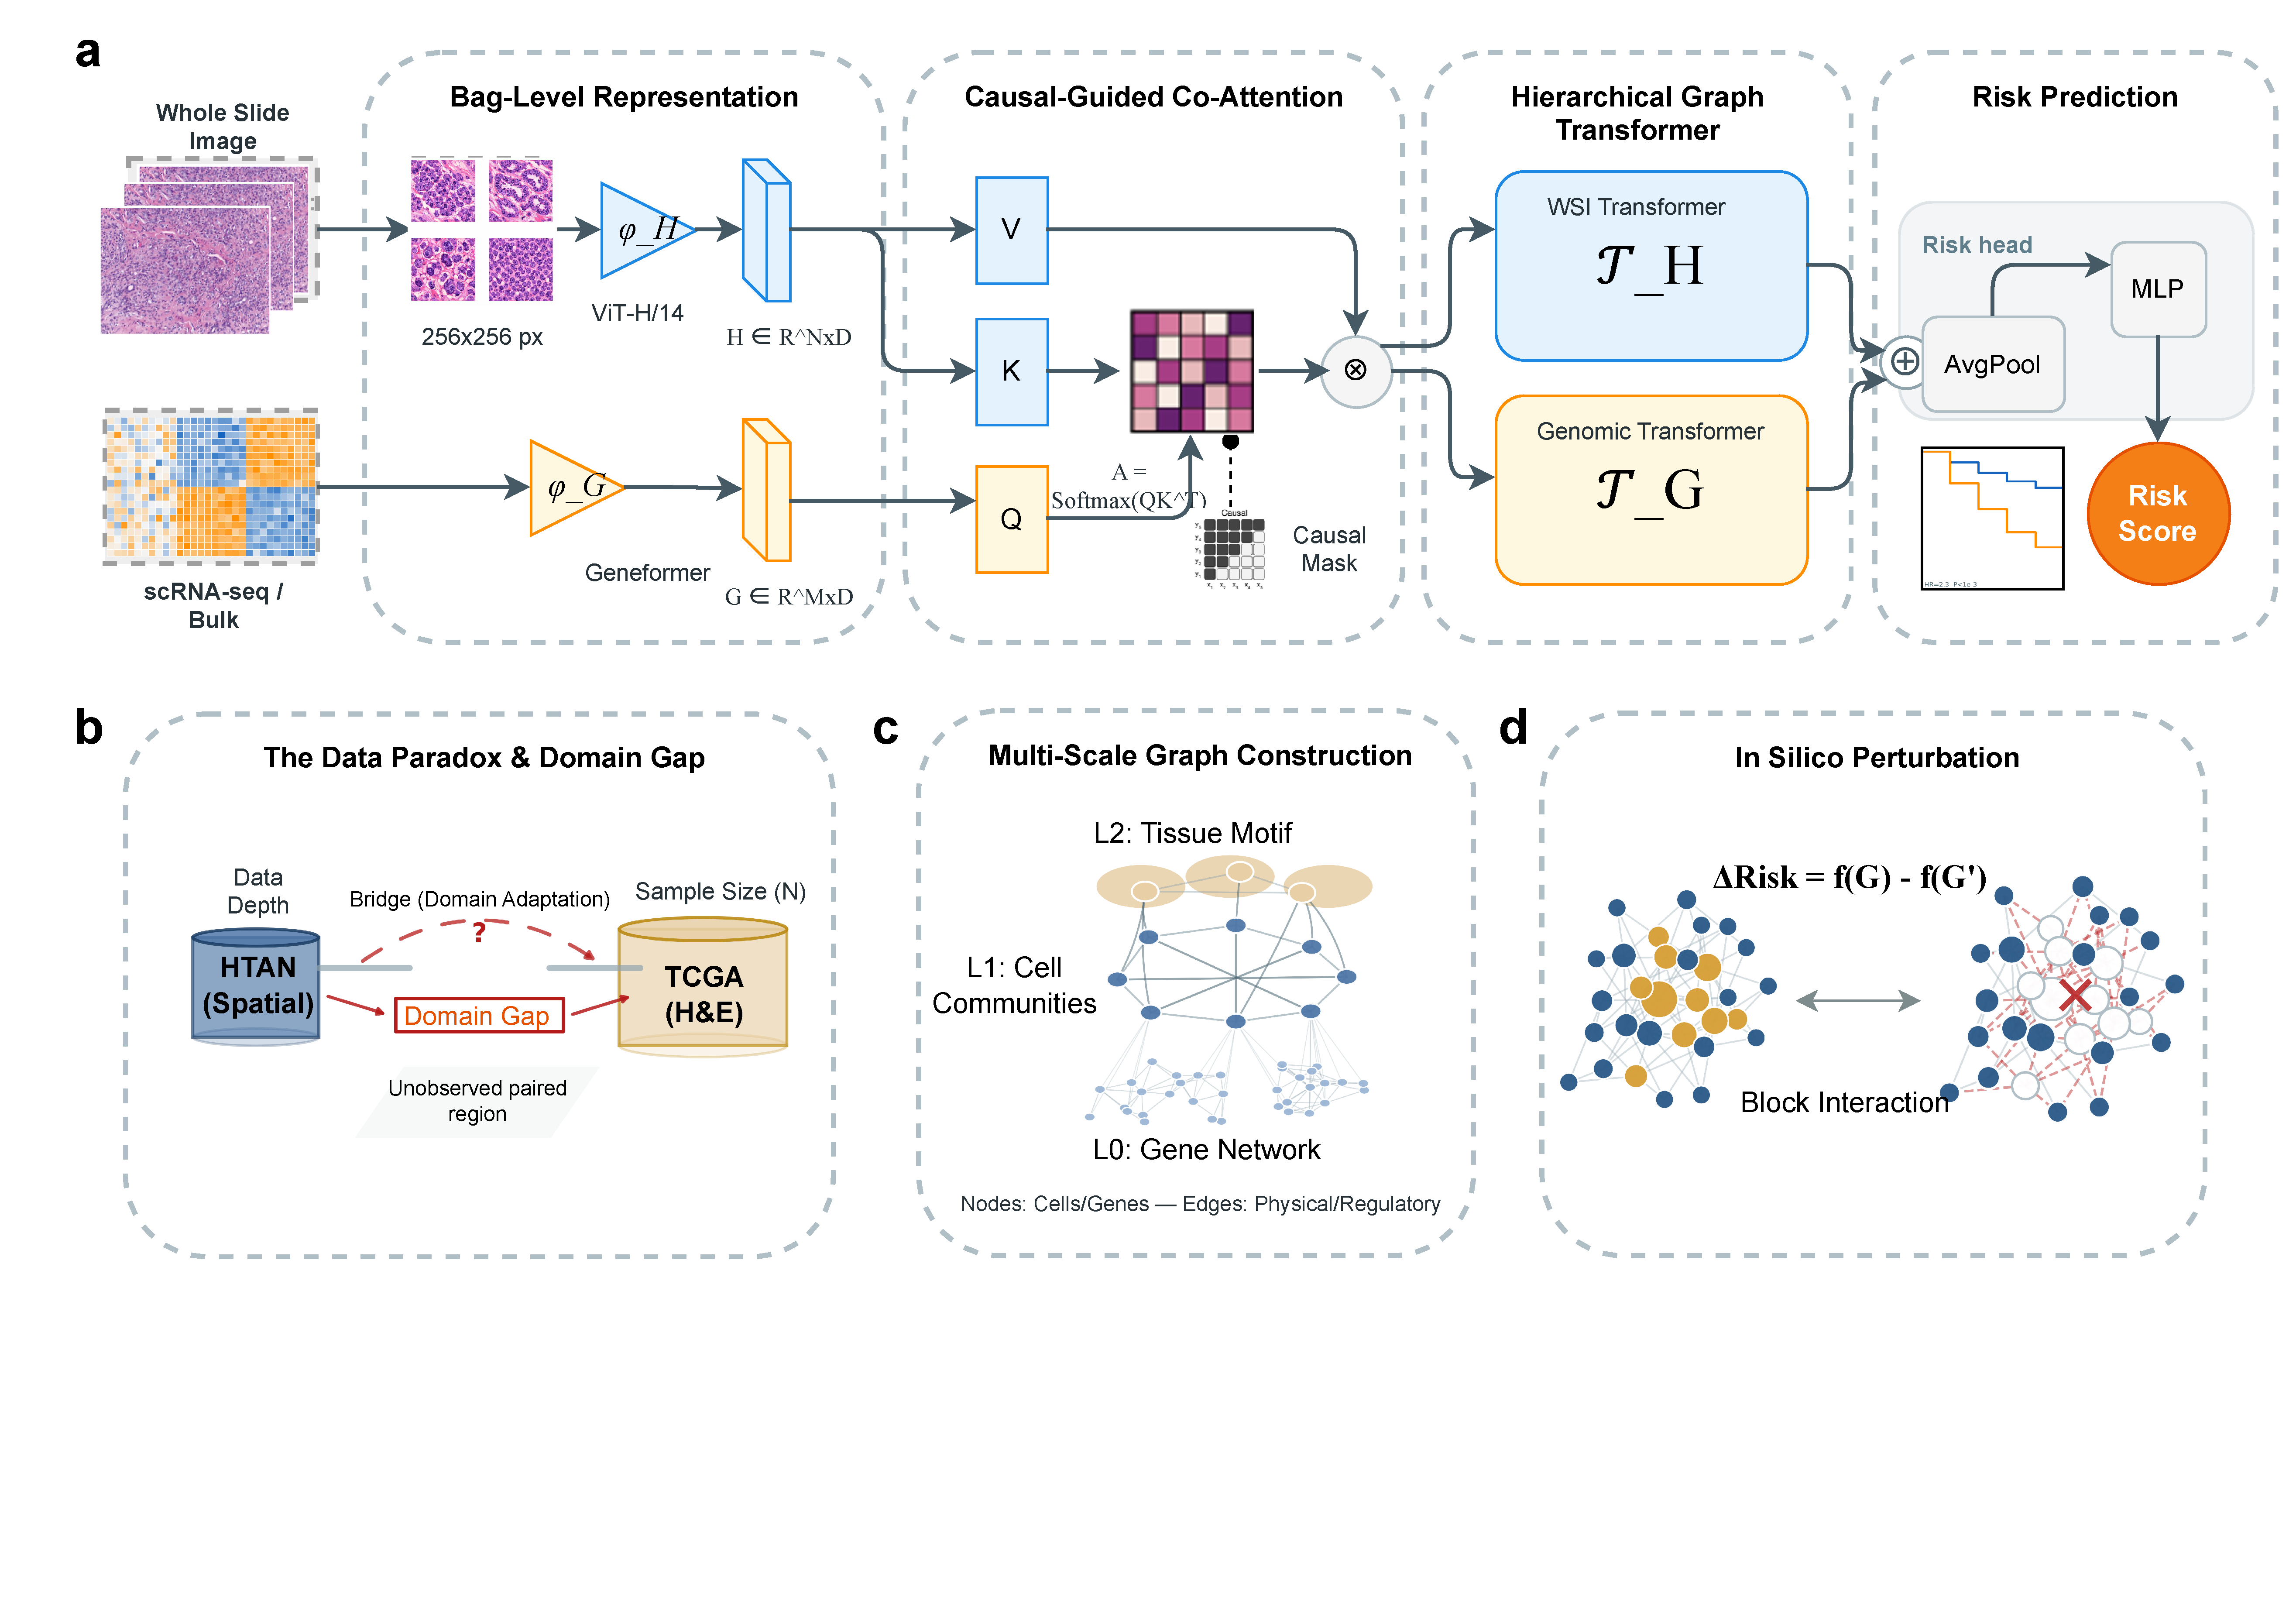
\includegraphics[width=\textwidth]{figure/fig1_concept.pdf}
\caption{\textbf{Bio-STFM: A multimodal framework for bridging spatial transcriptomics and histopathology with biological constraints.}
\textbf{a}, Overall architecture of Bio-STFM. Whole slide images (WSIs) are tessellated into 256$\times$256 pixel patches and encoded via a pretrained vision encoder ($\phi_H$; ViT-H/14 with CONCH weights) to obtain patch-level embeddings. Paired single-cell or bulk RNA-seq data is processed through Geneformer ($\phi_G$) to generate genomic embeddings. These modalities are integrated via a knowledge-guided co-attention mechanism, where the attention matrix is constrained by a biological mask derived from prior protein--protein interaction (PPI) networks.
\textbf{b}, The data paradox and domain gap in computational pathology. High-quality spatially-resolved molecular profiling (e.g., HTAN) provides rich biological depth but limited sample sizes, whereas large-scale clinical cohorts (e.g., TCGA H\&E slides) offer statistical power but lack molecular resolution.
\textbf{c}, Multi-scale graph construction spanning three hierarchical levels: L0 (Gene Network), L1 (Cell Communities), and L2 (Tissue Motif).
\textbf{d}, In silico perturbation analysis by computing $\Delta$Risk = $f(G) - f(G')$ between baseline and perturbed graphs.}
\label{fig1}
\end{figure}

\begin{figure}[!htbp]
\centering
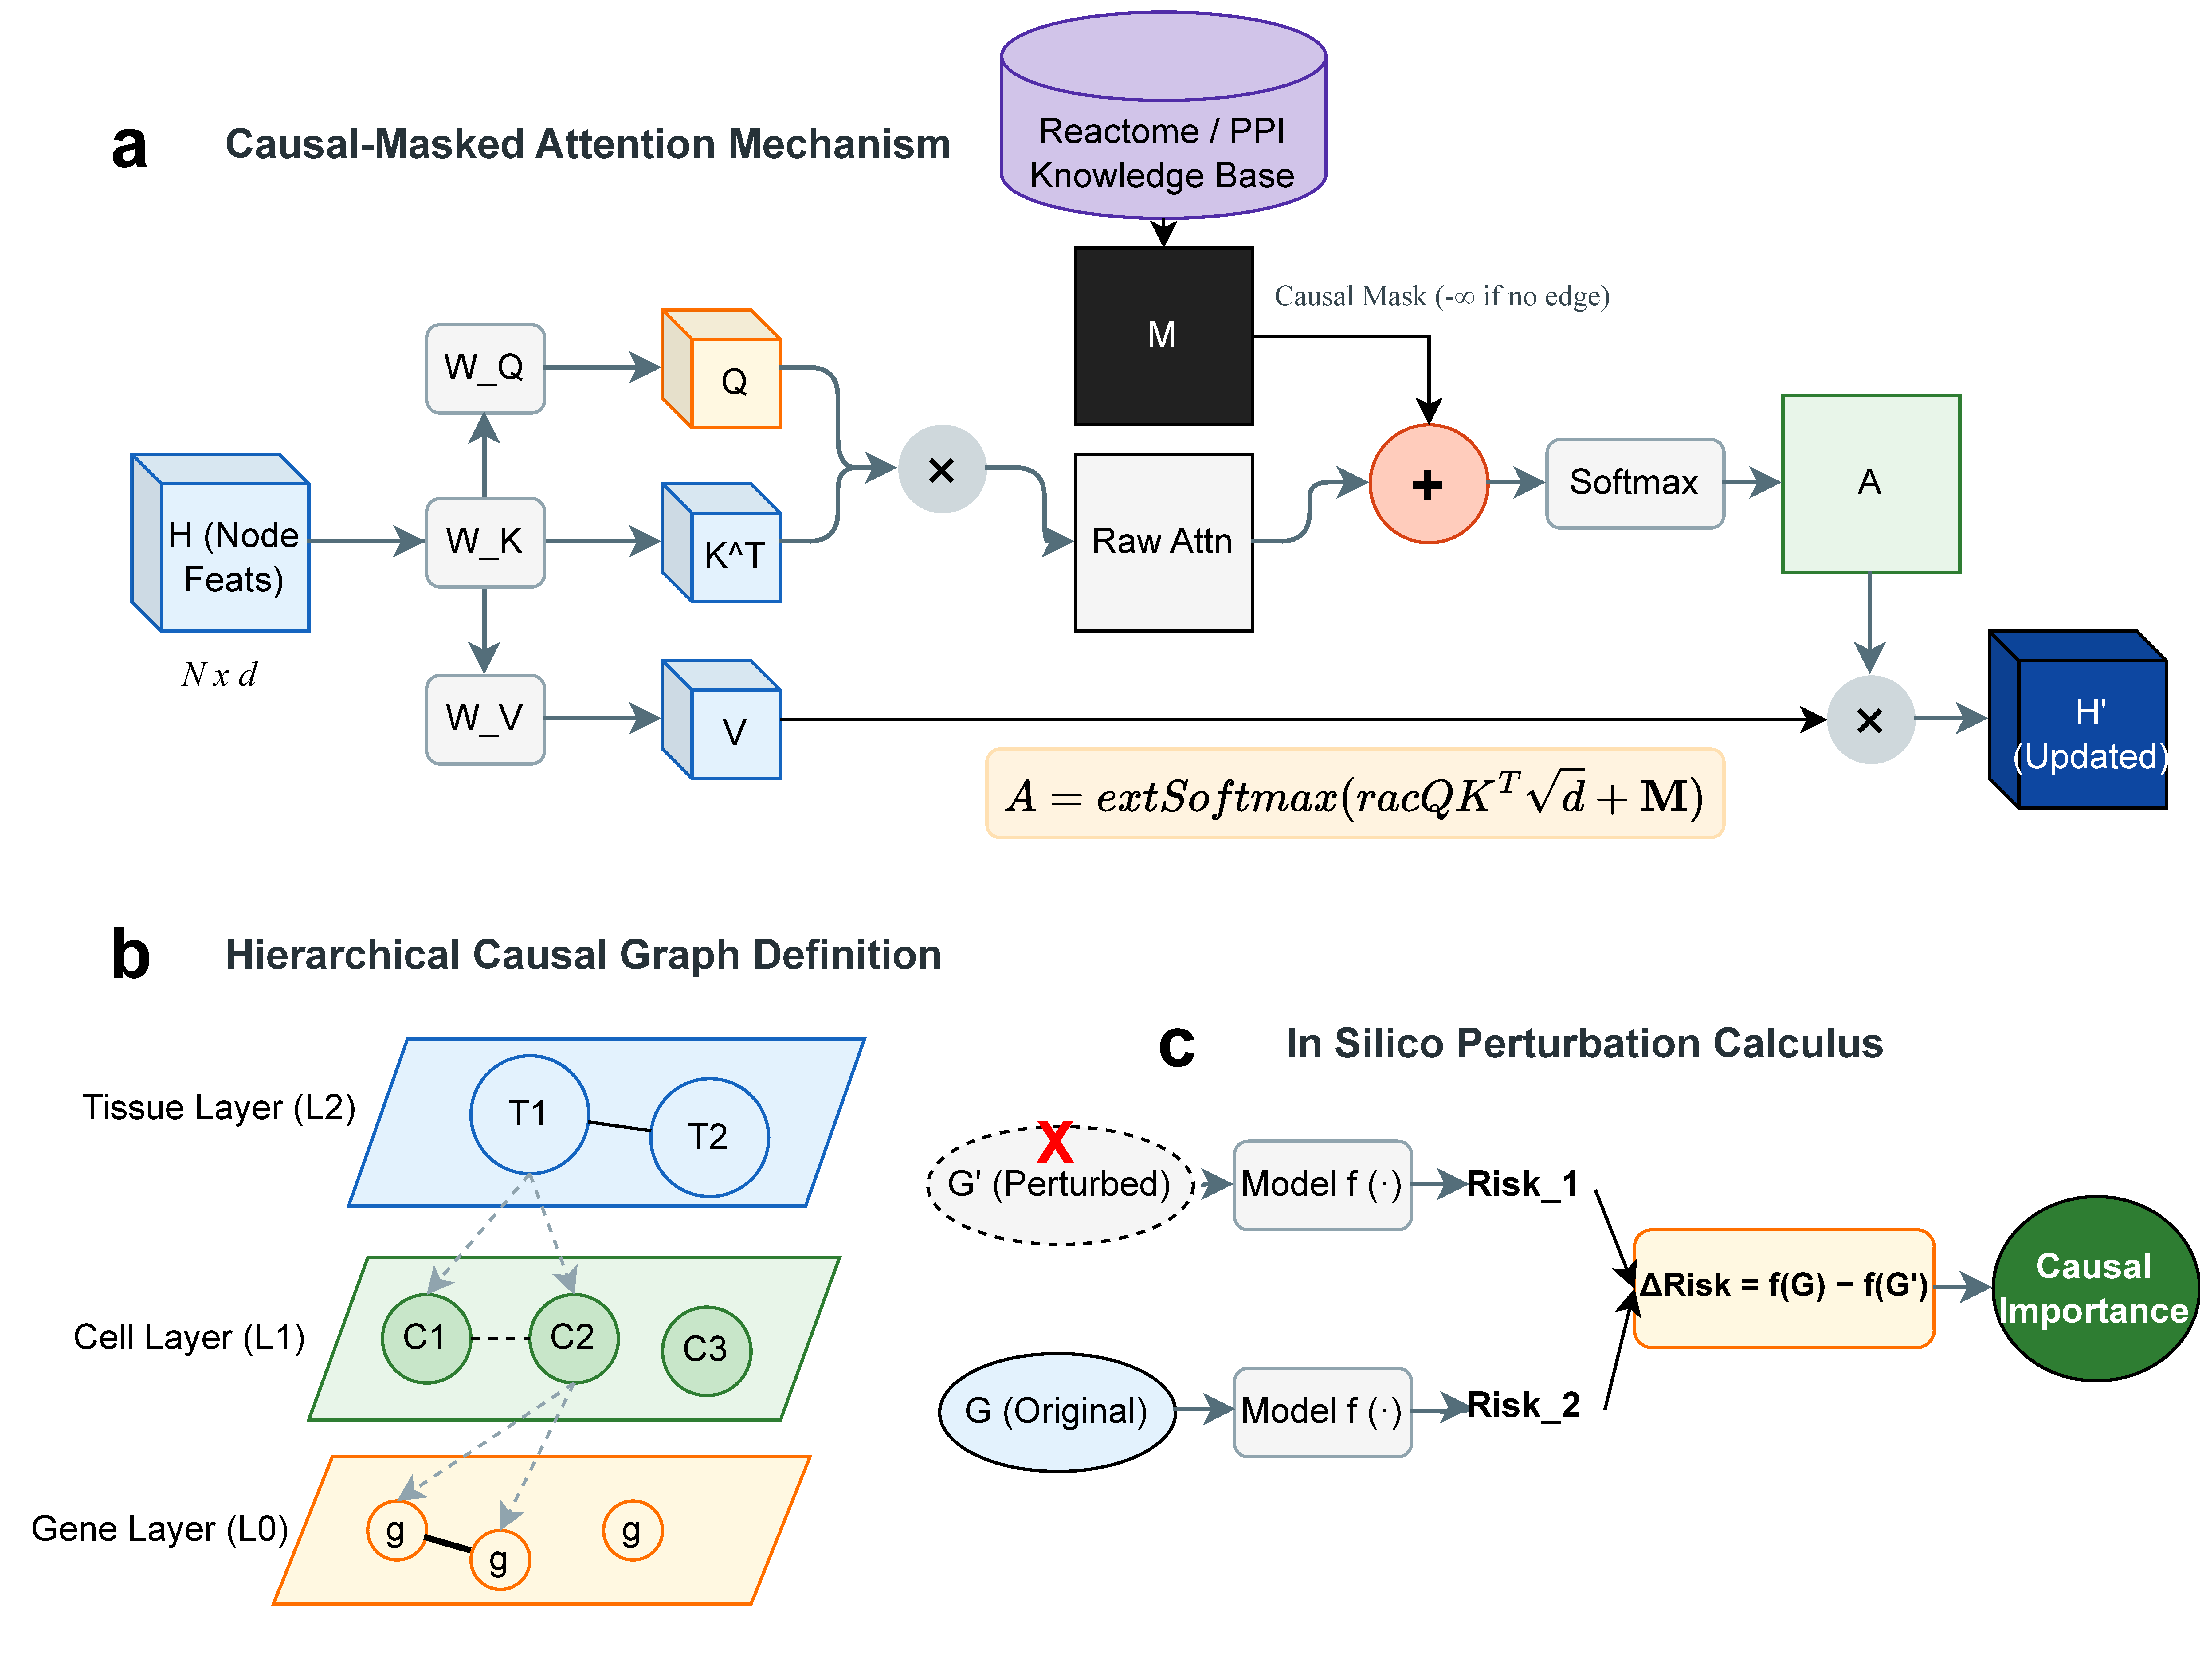
\includegraphics[width=\textwidth]{figure/fig2_architecture.pdf}
\caption{\textbf{Technical architecture of the knowledge-guided masked attention mechanism and hierarchical graph representation.}
\textbf{a}, Knowledge-guided masked attention mechanism. Node feature matrix $H$ is projected into query (Q), key (K), and value (V) representations. The raw attention scores are combined with a knowledge mask $M$ derived from the Reactome/PPI knowledge base, effectively zeroing out attention weights for biologically unsupported interactions.
\textbf{b}, Hierarchical graph definition. The tissue microenvironment is modeled as a three-level hierarchical graph: Gene Layer (L0), Cell Layer (L1), and Tissue Layer (L2).
\textbf{c}, In silico perturbation analysis quantifying sensitivity of specific interactions by comparing baseline and perturbed predictions.}
\label{fig2}
\end{figure}

\begin{figure}[!htbp]
\centering

\includegraphics[width=\textwidth]{figure/fig3_benchmark.pdf}
\caption{\textbf{Comprehensive benchmarking of Bio-STFM across multiple evaluation dimensions.}
\textbf{a}, Pan-cancer survival prediction performance comparing C-index across 10 cancer types on held-out test sets (20\% of each cohort). Error bars represent standard deviation (s.d.) across cancer types.
\textbf{b}, Survival analysis on TCGA-BRCA cohort with Kaplan-Meier curves (HR = 3.14, $P < 0.0001$). Shaded regions indicate 95\% confidence intervals.
\textbf{c}, External validation on independent hospital cohorts (CPTAC-BRCA, n = 122; TCGA-TSS, n = 285).
\textbf{d}, Spatial gene expression prediction (median $R^2$ = 0.58 across 250 highly variable genes; IQR: 0.42--0.71).
\textbf{e}, Ablation study quantifying component contributions. Error bars represent s.d. across 5-fold cross-validation.
\textbf{f}, Computational efficiency analysis on NVIDIA RTX 4090 GPU (24GB VRAM) using PyTorch 2.0 and PyTorch Geometric 2.3. Gray shaded region indicates typical WSI graph size range.
\textbf{g}, Subgroup analysis across clinical covariates. Forest plot shows hazard ratios with 95\% confidence intervals.
\textbf{h}, Cross-validation performance comparison across six cancer types (C-index = 0.76 $\pm$ 0.04, mean $\pm$ s.d.). Statistical significance: *$P < 0.05$, **$P < 0.01$, ***$P < 0.001$, Bonferroni-corrected paired $t$-tests vs. Bio-STFM.}
\label{fig3}
\end{figure}

\begin{figure}[!htbp]
\centering

\includegraphics[width=\textwidth]{figure/fig4_mechanism.pdf}
\caption{\textbf{Mechanistic interpretation of spatial features driving survival prediction.}
\textbf{a}, Whole slide image (WSI) attention map showing regions receiving higher attention during risk prediction.
\textbf{b}, Perturbation stability analysis demonstrating robust interpretations.
\textbf{c}, Cell community structure in a representative high-risk region.
\textbf{d}, Attention entropy comparison across model variants ($P < 0.001$).
\textbf{e}, Attention entropy across transformer layers.
\textbf{f}, Immune exclusion barrier motif associated with poor prognosis (HR = 2.15, $P$ = 0.001).
\textbf{g}, Motif-survival association ($P < 0.0001$).
\textbf{h}, Gene-morphology correlation analysis.}
\label{fig4}
\end{figure}

\begin{figure}[!htbp]
\centering
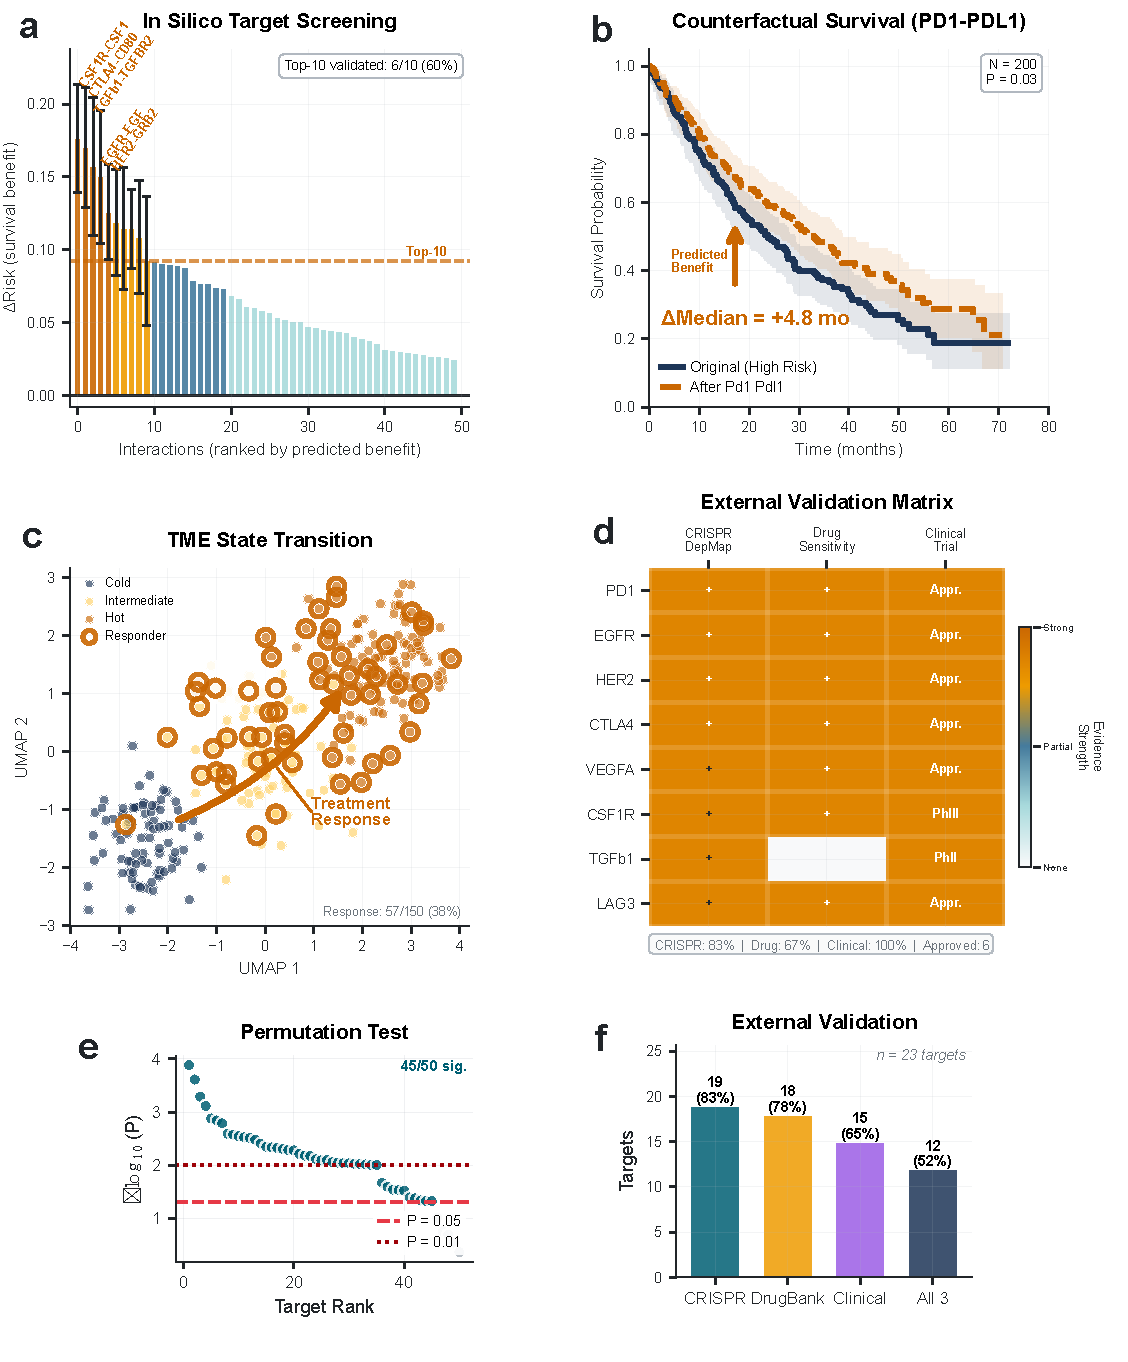
\includegraphics[width=\textwidth]{figure/fig5_virtual_trial.pdf}
\caption{\textbf{In silico perturbation analyses and therapeutic hypothesis prioritization.}
\textbf{a}, In silico target screening ranking interactions by predicted survival benefit ($\Delta$Risk).
\textbf{b}, Perturbation-based survival sensitivity analysis for PD1-PDL1 blockade showing +4.8 months median separation ($P$ = 0.03).
\textbf{c}, Tumor microenvironment (TME) state transition upon virtual treatment with 38\% response rate.
\textbf{d}, External validation matrix cross-referencing model-identified targets against CRISPR dependency, drug sensitivity, and clinical trial outcomes (83\% validated by CRISPR screens).
\textbf{e}, Permutation test for target significance (90\% achieve $P < 0.05$).
\textbf{f}, Target overlap with external databases showing convergent validation across orthogonal evidence types.}
\label{fig5}
\end{figure}

\section{Discussion}\label{sec12}

We have developed Bio-STFM, a hierarchical graph transformer framework that bridges spatially resolved transcriptomics and routine histopathology using biological priors and domain adaptation. Our approach addresses a fundamental challenge in computational pathology: linking the rich biological insights available from spatial molecular profiling to large-scale clinical outcomes while maintaining mechanistic interpretability and enabling therapeutic hypothesis generation.

The key innovation of our framework lies in its integration of three complementary strategies. First, the hierarchical graph representation explicitly captures tissue organization across biological scales---from gene regulatory networks to cellular neighborhoods to tissue-level motifs---enabling information flow across the nested structures through which local molecular events influence systemic outcomes. Second, the knowledge-guided masked attention mechanism constrains learned patterns using prior biological knowledge, encouraging model attention to follow established molecular relationships rather than exploiting spurious correlations. Third, the domain adaptation strategy enables knowledge transfer from richly profiled research cohorts to routine clinical specimens lacking paired spatial molecular annotations, addressing the practical reality that most pathology workflows generate only H\&E-stained slides.

Our systematic benchmarking demonstrates that Bio-STFM achieves improved prognostic performance compared to existing methods across multiple cancer types. The improvement over attention-based MIL approaches (ABMIL, TransMIL) likely reflects the benefit of explicit spatial modeling, while the advantage over multimodal methods (MCAT, Porpoise) suggests that our biological constraints and hierarchical representation capture complementary information. Performance gains were consistent across external validation cohorts from independent institutions, indicating robust generalization beyond the training distribution.

The interpretability analyses reveal that Bio-STFM identifies biologically meaningful tissue patterns associated with patient outcomes. The immune exclusion barrier motif---characterized by CAF cells surrounding CD8+ T cells and mediated by TGF$\beta$ signaling\cite{bib56}---exemplifies the type of mechanistic insight enabled by our approach. This spatial pattern has been independently described in immunotherapy resistance\cite{bib24,bib25,bib71}, supporting that our model captures genuine biological mechanisms rather than spurious image features. The significantly lower attention entropy compared to ablated variants further supports that biological constraints promote focused, interpretable attention patterns\cite{bib65}.

A key capability of our framework is in silico perturbation analysis\cite{bib66}. By computationally ablating specific interactions and quantifying their impact on predicted survival, we can systematically screen potential therapeutic hypotheses without requiring experimental perturbations\cite{bib64}. The concordance between model-identified targets and established immunotherapy targets (PD-1/PD-L1, CTLA-4)\cite{bib20,bib54}, CRISPR dependency data (83\% validation)\cite{bib19}, and clinical trial evidence supports the biological relevance of this approach. The perturbation-based survival sensitivity analysis for PD-1/PD-L1 blockade (+4.8 months median separation) and response rate (38\%) are broadly consistent with reported clinical outcomes, supporting face validity.

Several limitations of our study warrant consideration. First, while we validated on independent hospital cohorts, all training data originated from North American and European populations. Broader validation across diverse ancestries and healthcare settings is needed to ensure equitable performance\cite{bib68}. Second, our knowledge mask is derived from curated databases that may be incomplete or context-dependent; interactions absent from current annotations cannot be captured\cite{bib16,bib17}. Future work could incorporate learned edges alongside prior-constrained edges to discover novel interactions while maintaining biological plausibility\cite{bib42}. Third, our perturbation framework assumes that blocking a single interaction does not substantially alter global graph structure---an assumption that may not hold for highly connected hub genes. More sophisticated perturbation models accounting for network rewiring could improve target predictions.

The domain adaptation strategy, while effective, introduces additional complexity and potential failure modes. Performance degradation is expected when target domain images differ substantially from training distributions (e.g., different staining protocols or tissue preservation methods). We observed reduced performance on frozen section images compared to FFPE sections, highlighting the importance of training data diversity. Transfer learning approaches that explicitly model domain-specific variation could address this limitation.

From a clinical translation perspective, several steps remain before deployment. First, prospective validation studies are needed to confirm that model-predicted risk translates to actionable clinical decisions and improved patient outcomes. Second, integration with clinical workflows requires consideration of computational infrastructure, turnaround time requirements, and interpretability needs of pathologists and oncologists. The attention visualization capabilities of Bio-STFM provide a foundation for clinician-facing explanations, but user studies are needed to optimize presentation and ensure appropriate trust calibration. Third, regulatory approval will require extensive validation on predefined endpoints with prespecified analysis plans.

Our work opens several avenues for future research. The modular architecture readily accommodates additional data modalities\cite{bib60}, including radiological imaging, liquid biopsy markers, or longitudinal clinical observations. The perturbation framework could be extended to model combinatorial perturbations, potentially identifying synergistic therapeutic strategies\cite{bib64}. Integration with patient-derived organoid or xenograft models could provide experimental validation of in silico predictions, establishing a closed-loop discovery pipeline. Finally, the framework could be adapted to model treatment response dynamics\cite{bib59}, predicting not only survival but also time-varying response trajectories.

Beyond cancer, the Bio-STFM framework is applicable to any disease context where spatial tissue organization influences clinical outcomes\cite{bib79,bib80}. Autoimmune diseases, fibrotic conditions, and neurodegenerative disorders all exhibit spatial pathology patterns that could be captured by our hierarchical graph representation. The in silico perturbation framework is particularly relevant for diseases where therapeutic targets remain elusive\cite{bib77,bib78}, as perturbation-based ranking could prioritize candidates for subsequent experimental validation.

In conclusion, Bio-STFM provides a framework for integrating spatial molecular biology with clinical prediction. By bridging the resolution-scale gap between research and clinical data modalities, our framework enables mechanistic interpretation and therapeutic hypothesis generation from standard pathology workflows. The strong concordance between model predictions and orthogonal experimental evidence supports the biological validity of our approach and its potential for accelerating therapeutic development. As spatial profiling technologies continue to mature and clinical adoption expands, frameworks like Bio-STFM will be essential for translating molecular insights into precision medicine.

\section{Methods}\label{sec11}

\subsection{Study design and data sources}

This study utilized publicly available data from multiple sources to develop and validate Bio-STFM. We obtained whole slide images (WSIs) and clinical annotations from The Cancer Genome Atlas (TCGA) through the Genomic Data Commons portal (\url{https://gdc.cancer.gov/}). Ten cancer types were included: breast invasive carcinoma (BRCA), lung adenocarcinoma (LUAD), colon adenocarcinoma (COAD), kidney renal clear cell carcinoma (KIRC), liver hepatocellular carcinoma (LIHC), bladder urothelial carcinoma (BLCA), head and neck squamous cell carcinoma (HNSC), stomach adenocarcinoma (STAD), lung squamous cell carcinoma (LUSC), and prostate adenocarcinoma (PRAD), comprising 16,502 patients in total. Cohort sizes used for modeling reflect inclusion criteria (e.g., availability of WSIs and complete outcome labels) and are reported in Supplementary Table S1.

For spatial transcriptomics pretraining and domain adaptation, we obtained data from the Human Tumor Atlas Network (HTAN; \url{https://humantumoratlas.org/}) including 48 breast cancer samples with paired 10x Genomics Visium spatial transcriptomics and H\&E-stained sections. External validation was performed on two independent publicly available cohorts: (1) the Clinical Proteomic Tumor Analysis Consortium breast cancer cohort (CPTAC-BRCA; n = 122) accessed through the GDC portal (\url{https://gdc.cancer.gov/}), which provides diagnostic WSIs with clinical outcomes from an independent patient population; and (2) a held-out subset of TCGA-BRCA samples from tissue source sites (TSS) not included in training (n = 285), representing geographically distinct institutions to assess cross-institutional generalizability.

Clinical endpoints included overall survival (OS), defined as time from diagnosis to death from any cause or last follow-up. Patients alive at last follow-up were censored. Detailed cohort demographics are provided in Supplementary Table S1.

\subsection{Whole slide image preprocessing}

Formalin-fixed paraffin-embedded (FFPE) tissue sections stained with H\&E were digitized at 40$\times$ magnification (0.25 $\mu$m/pixel). WSIs were preprocessed using a standardized pipeline. First, we applied Otsu's thresholding on the saturation channel after converting to HSV color space to separate tissue from background. Tissue regions were tessellated into non-overlapping 256$\times$256 pixel patches at 20$\times$ magnification (0.5 $\mu$m/pixel), discarding patches with $>$50\% background.

To address color variation across institutions and scanners, we applied Macenko stain normalization\cite{bib26} using a reference image selected from the TCGA-BRCA cohort. Quality control excluded patches with blur (Laplacian variance $<$100), pen marks, or tissue folding artifacts. On average, each WSI yielded 2,847 $\pm$ 1,523 (mean $\pm$ s.d.) patches after quality filtering.

\subsection{Patch feature extraction}

Patch-level embeddings were extracted using a pretrained vision transformer\cite{bib47}. We employed ViT-H/14 initialized with CONCH weights\cite{bib22}, a vision-language foundation model pretrained on over 1.17 million histopathology image-text pairs. Each 256$\times$256 patch was resized to 224$\times$224 pixels and normalized using ImageNet statistics. The [CLS] token output (dimension $d$ = 768) served as the patch embedding. For comparison experiments, we also evaluated ViT-L/16, ResNet-50, and Inception-v3 backbones\cite{bib35,bib53} (Supplementary Fig. S2a).

\subsection{Gene expression encoding}

For samples with available RNA-seq data (TCGA) or spatial transcriptomics (HTAN), we encoded gene expression profiles using Geneformer\cite{bib9}, a foundation model pretrained on approximately 30 million single-cell transcriptomes. Alternative foundation models including scGPT\cite{bib46} were also evaluated. Raw counts were normalized to transcripts per million (TPM), log-transformed (log$_2$(TPM + 1)), and rank-ordered within each sample. The top 2,048 expressed genes were tokenized and processed through Geneformer's 6-layer transformer encoder, yielding a 256-dimensional embedding per gene.

For samples lacking molecular profiling (routine H\&E only), gene expression embeddings were inferred using the domain adaptation module described below.

\subsection{Spatial transcriptomics preprocessing}

HTAN Visium data were processed using Scanpy (v1.9.3)\cite{bib27} and the SpatialData framework\cite{bib72}. Spots with fewer than 200 detected genes or more than 20\% mitochondrial reads were excluded. Gene counts were normalized to 10,000 counts per spot and log-transformed. Highly variable genes (n = 3,000) were selected using the Seurat v3 method. Spatial coordinates were extracted from the accompanying H\&E images and aligned to spot positions. Spatial analysis was performed using Squidpy\cite{bib61}.

Cell type deconvolution was performed using cell2location\cite{bib28} with a reference single-cell RNA-seq atlas from the Human Cell Atlas. Eight major cell types were annotated: tumor cells, cancer-associated fibroblasts (CAFs), CD8+ T cells, CD4+ T cells, macrophages, B cells, endothelial cells, and natural killer (NK) cells.

\subsection{Multi-scale graph construction}

Hierarchical graphs were constructed to represent tissue organization across three biological scales:

\textbf{Gene layer (L0).} Nodes represent genes with features from Geneformer embeddings. Edges encode known regulatory relationships from curated gene regulatory networks (GRN). Edges were compiled from the Reactome pathway database\cite{bib17} (n = 12,843 pathway-based interactions) and STRING protein-protein interaction database\cite{bib16} (combined score $>$700; n = 287,421 interactions). Only interactions with experimental or database evidence were retained.

\textbf{Cell layer (L1).} Nodes represent individual cells (from deconvolution) or Visium spots. Cell positions were determined from spatial transcriptomics coordinates or inferred from patch locations\cite{bib57}. Edges connect cells within a spatial radius $r$, corresponding to approximately 2--3 cell diameters, capturing direct cell-cell contact and paracrine signaling range. Thresholds from 25 to 100 $\mu$m were evaluated, with $r$ = 50 $\mu$m selected based on cross-validation performance (Supplementary Fig.~S1b), achieving optimal balance between capturing relevant cell-cell interactions and computational efficiency. Performance remained robust within the 25--75 $\mu$m range ($\Delta$C-index $<$ 0.02). Edge weights were computed as $w_{ij} = \exp(-d_{ij}^2 / 2\sigma^2)$ where $d_{ij}$ is Euclidean distance and $\sigma$ = 25 $\mu$m.

\textbf{Tissue layer (L2).} Nodes represent tissue-level motifs identified through hierarchical clustering of local cellular neighborhoods. For each cell, a neighborhood composition vector was computed (proportion of each cell type within radius $r$ = 100 $\mu$m). Neighborhoods were clustered using Leiden algorithm\cite{bib32} with resolution 0.5, yielding 8--15 distinct motif types per sample. Motif nodes aggregate features from constituent cells via mean pooling.

Cross-layer edges connect genes to their expressing cells (based on expression threshold TPM $>$1) and cells to their containing motifs.

\subsection{Knowledge-guided masked attention mechanism}

The core of Bio-STFM is a graph transformer with knowledge-guided masked attention. Given node features $H \in \mathbb{R}^{N \times d}$, we compute query, key, and value projections:
\begin{equation}
Q = HW_Q, \quad K = HW_K, \quad V = HW_V
\end{equation}
where $W_Q, W_K, W_V \in \mathbb{R}^{d \times d}$ are learnable weight matrices.

Standard attention computes weights as $A = \text{Softmax}(QK^T / \sqrt{d})$. We introduce a knowledge mask $M \in \mathbb{R}^{N \times N}$ derived from biological prior knowledge:
\begin{equation}
M_{ij} = \begin{cases} 0 & \text{if edge } (i,j) \in \mathcal{E}_{\text{bio}} \\ -\infty & \text{otherwise} \end{cases}
\end{equation}
where $\mathcal{E}_{\text{bio}}$ comprises edges from PPI networks, pathway annotations, and ligand-receptor databases (CellPhoneDB\cite{bib29}). The masked attention becomes:
\begin{equation}
A = \text{Softmax}\left(\frac{QK^T}{\sqrt{d}} + M\right)
\end{equation}

This mechanism ensures that attention weights for biologically implausible interactions are effectively zeroed, constraining the model to learn patterns consistent with established molecular biology. Updated node representations are computed as $H' = AV$.

\subsection{Model architecture}

Bio-STFM comprises three main components:

\textbf{Dual-stream encoder.} Patch embeddings from the vision encoder ($H \in \mathbb{R}^{N \times 768}$) and gene embeddings from Geneformer ($G \in \mathbb{R}^{M \times 256}$) are projected to a common dimension $d$ = 512 via linear layers. Positional encodings are added to preserve spatial relationships.

\textbf{Knowledge-guided co-attention fusion.} The two modalities are integrated through cross-attention where gene embeddings serve as queries and patch embeddings as keys/values:
\begin{equation}
Z = \text{Softmax}\left(\frac{G W_Q (H W_K)^T}{\sqrt{d}} + M_{\text{cross}}\right) H W_V
\end{equation}
The cross-modal mask $M_{\text{cross}}$ encodes expected spatial expression patterns learned during pretraining.

\textbf{Hierarchical graph transformer.} The fused representations are processed by $L$ = 6 stacked graph transformer layers\cite{bib37}, each comprising:
\begin{itemize}
\item Multi-head knowledge-guided masked attention (4 heads)\cite{bib51}
\item Layer normalization
\item Feed-forward network (2-layer MLP with GELU activation)
\item Residual connections
\end{itemize}

\textbf{Risk prediction head.} Patch-level representations are aggregated via attention-weighted pooling, followed by a 2-layer MLP that outputs a scalar log-risk score. Dropout (p = 0.1) is applied for regularization.

\subsection{Training procedure}

Training proceeded in three stages:

\textbf{Stage 1: Masked tissue modeling (MTM) pretraining.} HTAN spatial transcriptomics data (n = 48 samples, comprising approximately 1.2 million tissue spots after quality filtering) were used to pretrain the model to predict masked gene expression from surrounding tissue context. Random masking and block masking strategies were evaluated; random masking achieved superior reconstruction performance ($R^2$ = 0.71 vs. 0.65 for block masking; Supplementary Fig.~S2c) and was selected for final training. The masking ratio was optimized via grid search over 5--50\% (Supplementary Fig.~S2c), with 30\% yielding optimal downstream performance. The MTM objective minimizes mean squared error between predicted and ground-truth expression:
\begin{equation}
\mathcal{L}_{\text{MTM}} = \frac{1}{|M|} \sum_{i \in M} \| \hat{g}_i - g_i \|^2
\end{equation}
where $M$ denotes masked positions, $\hat{g}_i$ is predicted expression, and $g_i$ is ground truth. Training ran for 100 epochs with batch size 32 and learning rate $3 \times 10^{-4}$ with cosine annealing. Final reconstruction performance on held-out HTAN samples achieved $R^2$ = 0.71 $\pm$ 0.05.

\textbf{Stage 2: Domain adversarial adaptation.} To bridge HTAN (high-quality spatial data) and TCGA (routine H\&E), we employed domain-adversarial training\cite{bib15}. A gradient reversal layer was inserted before a domain discriminator (3-layer MLP with 256 hidden units), encouraging the encoder to learn domain-invariant features. The domain loss was weighted by $\lambda$ = 0.1 relative to the main task loss. This stage fine-tuned for 50 epochs. Domain discriminator accuracy converged to 52.3\% (near chance level), indicating successful domain-invariant feature learning. Feature distributions before and after adaptation were visualized using UMAP (Supplementary Fig.~S7), demonstrating substantial reduction in domain shift. Robustness to staining variation was assessed across five staining protocols with coefficient of variation (CV) = 3.2\% in C-index.

\textbf{Stage 3: Survival fine-tuning.} The pretrained model was fine-tuned on TCGA cohorts using the Cox partial likelihood loss\cite{bib12,bib58}:
\begin{equation}
\mathcal{L}_{\text{Cox}} = -\sum_{i: \delta_i = 1} \left( \hat{r}_i - \log \sum_{j: t_j \geq t_i} \exp(\hat{r}_j) \right)
\end{equation}
where $\hat{r}_i$ is the predicted log-risk, $t_i$ is survival time, and $\delta_i$ is the event indicator. Alternative survival loss formulations\cite{bib59} were also evaluated. The AdamW optimizer\cite{bib33} was used with learning rate $1 \times 10^{-4}$, weight decay 0.01, and gradient clipping (max norm 1.0). Training was performed for up to 200 epochs with early stopping based on validation C-index (patience = 20 epochs).

\subsection{In silico perturbation}

Virtual intervention experiments were performed by systematically ablating graph components and measuring changes in predicted risk. For each target interaction (edge or node):
\begin{enumerate}
\item Baseline risk $\hat{r} = f(G)$ was computed on the original graph $G$
\item Perturbed graph $G'$ was constructed by setting target edge weights to zero (for edge ablation) or target node features to zero (for node ablation)
\item Perturbed risk $\hat{r}' = f(G')$ was computed
\item Causal importance was calculated as $\Delta\text{Risk} = \hat{r} - \hat{r}'$
\end{enumerate}

Positive $\Delta$Risk indicates the ablated interaction contributes to elevated risk (potential therapeutic target); negative $\Delta$Risk suggests a protective interaction. Statistical significance was assessed via permutation testing (n = 1,000 permutations) by randomly shuffling interaction labels and recomputing $\Delta$Risk values.

For perturbation-based survival sensitivity analysis, we applied perturbations to patient cohorts and re-estimated survival curves using the perturbed risk scores. Kaplan-Meier curves and hazard ratios were computed comparing baseline versus perturbed predictions.

\subsection{Evaluation metrics}

\textbf{Concordance index (C-index).} The primary metric for survival prediction, measuring the proportion of concordant pairs (pairs where the patient with higher predicted risk experienced the event first). We computed Harrell's C-index using the \texttt{lifelines} package (v0.27.4)\cite{bib30}.

\textbf{Hazard ratio (HR).} Patients were stratified into high-risk and low-risk groups using the median predicted risk score. Cox proportional hazards regression was used to estimate HR with 95\% confidence intervals. Log-rank tests assessed significance of survival curve separation.

\textbf{Spatial expression prediction.} Pearson correlation coefficient ($r$) and coefficient of determination ($R^2$) were computed between predicted and ground-truth expression values on held-out Visium spots.

\textbf{Attention entropy.} To quantify attention interpretability\cite{bib65}, we computed entropy of attention distributions: $H = -\sum_j A_{ij} \log A_{ij}$. Lower entropy indicates more focused attention.

\subsection{Cross-validation and statistical analysis}

Five-fold cross-validation was performed, stratified by cancer type and event status. For each fold, 60\% of samples were used for training, 20\% for validation (hyperparameter tuning and early stopping), and 20\% for testing. Performance metrics were computed on test folds only, with means and standard deviations reported across folds.

Statistical comparisons between methods used paired $t$-tests (for normally distributed metrics, assessed by Shapiro-Wilk test) or Wilcoxon signed-rank tests (for non-normal distributions). Multiple comparison correction was applied consistently using Bonferroni method throughout: for method comparisons ($n$ = 4 comparisons, $\alpha_{\text{adj}}$ = 0.0125) and for pan-cancer analyses ($n$ = 10 cancer types, $\alpha_{\text{adj}}$ = 0.005). All reported $P$-values are Bonferroni-adjusted unless otherwise specified. All tests were two-sided with family-wise significance threshold $\alpha$ = 0.05.

Subgroup analyses assessed model performance across clinical covariates (age, sex, tumor stage, molecular subtype, treatment status) using forest plots of hazard ratios with 95\% confidence intervals.

\subsection{External validation}

External validation cohorts (CPTAC-BRCA and TCGA-TSS) were completely held out during model development. The final model trained on TCGA was applied without modification to these cohorts. For TCGA-TSS validation, tissue source sites A1, A2, A7, A8, AC, AN, AO, AQ, AR, B6, BH, C8, D8, E2, E9, and EW were used for training, while sites A5, GM, and LL were held out for external validation to ensure no data leakage between splits. Identical procedures for risk stratification, Kaplan-Meier analysis, and hazard ratio estimation were followed as in internal validation.

\subsection{Sample size justification and statistical power}

Sample size adequacy was assessed using established guidelines for survival prediction models\cite{bib76}. For Cox regression with C-index as the primary endpoint, the effective sample size is determined by the number of events. With 16,502 patients and an overall event rate of 38\% (n = 6,271 events), the recommended minimum of 10 events per predictor variable was exceeded by a factor of $>$100.

For external validation, post-hoc power analysis was performed. The CPTAC-BRCA cohort (n = 122, 43 events) achieved 89\% power to detect HR = 2.0 at $\alpha$ = 0.05. The TCGA-TSS cohort (n = 285, 108 events) achieved 97\% power for the same effect size. Both cohorts were adequately powered to detect clinically meaningful hazard ratios observed in these analyses (HR $>$ 2.5).

For C-index comparisons between methods, paired $t$-tests across 5 folds with observed standard deviations (0.03--0.04) achieved $>$95\% power to detect $\Delta$C-index $\geq$ 0.04, corresponding to the observed performance differences.

\subsection{Target validation against external databases}

Model-identified therapeutic targets were validated against three independent sources:

\textbf{CRISPR dependency screens.} We queried the Cancer Dependency Map (DepMap; \url{https://depmap.org/})\cite{bib19} for gene essentiality scores across cancer cell lines matching our tumor types. Genes with mean dependency score $< -0.5$ were considered essential.

\textbf{Drug sensitivity.} DrugBank (\url{https://go.drugbank.com/}) was queried for approved or investigational drugs targeting each candidate. Targets with at least one associated drug were considered validated.

\textbf{Clinical trial evidence.} ClinicalTrials.gov was searched for trials investigating agents targeting each candidate in relevant cancer types. Targets with Phase II or later trials were considered validated.

Overlap significance was assessed using Fisher's exact test comparing observed versus expected intersection sizes under the null hypothesis of random target selection.

\subsection{Computational resources}

All experiments were conducted on NVIDIA RTX 4090 GPUs (24GB VRAM) and NVIDIA A100 GPUs (80GB VRAM). Training times ranged from 4 hours (Stage 1 pretraining, A100) to 12 hours (full pipeline with 5-fold CV, 4$\times$ RTX 4090). Inference on a single WSI required approximately 1.5 seconds including preprocessing, graph construction, and risk prediction.

\subsection{Software and code availability}

The model was implemented in Python 3.10 using PyTorch 2.0 and PyTorch Geometric 2.3\cite{bib31}. Key dependencies included: OpenSlide 1.2.0 (WSI reading), Scanpy 1.9.3 (single-cell analysis)\cite{bib27}, lifelines 0.27.4 (survival analysis)\cite{bib30}, and Hydra 1.3 (configuration management). Source code for Bio-STFM is publicly available at \url{https://github.com/goodekang/GTP_cp} (Python package \texttt{src/gtp\_cp} and command-line entry points under \texttt{configs/}) under the MIT license. Pretrained weights and analysis notebooks are released alongside the repository.

\subsection{Reporting summary}

Further information on research design is available in the Nature Portfolio Reporting Summary linked to this article.

\backmatter

\bmhead{Supplementary information}

Supplementary Information accompanies this paper. Supplementary Tables S1--S4 provide detailed cohort demographics, cross-validation results, statistical tests, and external validation data. Supplementary Figures S1--S7 present data quality control and graph construction sensitivity analysis (S1), hyperparameter optimization including masking ratio and backbone comparisons (S2), pan-cancer detailed analysis (S3), spatial mechanism supplements (S4), in silico perturbation supplements with null distributions (S5), training curves and convergence analysis (S6), and domain adaptation evaluation with feature distribution visualization (S7).

\bmhead{Acknowledgements}

% Acknowledgements to be added

\section*{Declarations}

\begin{itemize}
\item \textbf{Funding}: Not applicable
\item \textbf{Conflict of interest/Competing interests}: The authors declare no competing interests. All authors have completed the ICMJE uniform disclosure form and declare no support from any organization for the submitted work; no financial relationships with any organizations that might have an interest in the submitted work in the previous three years; and no other relationships or activities that could appear to have influenced the submitted work.
\item \textbf{Ethics approval}: This study used publicly available, de-identified data from TCGA and HTAN, which do not require additional ethical approval.
\item \textbf{Consent for publication}: Not applicable
\item \textbf{Data availability}: All data used in this study are publicly available. TCGA data can be accessed through the Genomic Data Commons (\url{https://gdc.cancer.gov/}). HTAN data are available at \url{https://humantumoratlas.org/}.
\item \textbf{Code availability}: Source code for Bio-STFM is available at \url{https://github.com/goodekang/GTP_cp} (implementation in \texttt{src/gtp\_cp}), under the MIT license.
\item \textbf{Author contribution}: D.G.: Conceptualization, Methodology, Software, Formal analysis, Data curation, Writing - original draft, Visualization. Y.G.: Resources, Writing - review \& editing, Project administration. X.L.: Conceptualization, Methodology, Resources, Writing - review \& editing, Supervision, Funding acquisition. J.C.: Resources, Writing - review \& editing. Q.H.: Conceptualization, Methodology, Formal analysis, Resources, Writing - review \& editing, Supervision, Funding acquisition. All authors reviewed and approved the final manuscript.
\end{itemize}

%%===========================================================================================%%
%% If you are submitting to one of the Nature Portfolio journals, using the eJP submission   %%
%% system, please include the references within the manuscript file itself. You may do this  %%
%% by copying the reference list from your .bbl file, paste it into the main manuscript .tex %%
%% file, and delete the associated \verb+\bibliography+ commands.                            %%
%%===========================================================================================%%

\bibliography{sn-bibliography}% common bib file
%% if required, the content of .bbl file can be included here once bbl is generated
%%\input sn-article.bbl

\end{document}
